\documentclass[a4paper,11pt]{article}

% --- PACKAGES DE BASE ---
\usepackage[utf8]{inputenc}
\usepackage[T1]{fontenc}
\usepackage[french]{babel}
\usepackage{geometry}
\usepackage{float}
\geometry{hmargin=2cm,vmargin=2cm}

% --- PACKAGES TECHNIQUES ---
\usepackage{graphicx}  % Pour insérer les graphiques de Bode et de filtrage spatial
\usepackage{amsmath}   % Pour les équations mathématiques complexes (Jacobienne, impédances)
\usepackage{amssymb}   % Pour les symboles mathématiques
\usepackage{booktabs}  % Pour faire de beaux tableaux de données numériques
\usepackage{listings}  % Pour insérer proprement tes fonctions Python
\usepackage{xcolor}    % Pour la coloration syntaxique du code
\usepackage{hyperref}  % Pour les liens internes et la table des matières cliquable
\usepackage{tabularx}

% --- CONFIGURATION DE LISTINGS (POUR PYTHON) ---
\definecolor{darkgray}{rgb}{0.3, 0.3, 0.3}
\definecolor{navyblue}{rgb}{0.0, 0.2, 0.6}
\definecolor{darkgreen}{rgb}{0.1, 0.4, 0.1}

\lstset{
    backgroundcolor=,                      % Supprime complètement le fond
    frame=single,                          % Cadre simple autour du code
    commentstyle=\color{darkgray}\itshape, % Commentaires gris discrets
    keywordstyle=\color{navyblue}\bfseries,% Mots-clés bleu sobre
    stringstyle=\color{darkgreen},         % Chaînes de caractères vertes calmes
    basicstyle=\ttfamily\scriptsize,       % Taille adaptée pour le code
    breaklines=true,                 
    numbers=left,                          % Garde les numéros à gauche
    numberstyle=\tiny\color{lightgray},    % Numéros très clairs
    tabsize=2,                             % Indentation compacte
    showstringspaces=false,
    inputencoding=utf8,
    extendedchars=true,
    literate=
        {é}{{\'e}}1 {è}{{\`e}}1 {à}{{\`a}}1 {ù}{{\`u}}1 {ç}{{\c{c}}}1
        {ê}{{\^e}}1 {â}{{\^a}}1 {î}{{\^i}}1 {ô}{{\^o}}1 {û}{{\^u}}1
        {ë}{{\"e}}1 {ï}{{\"i}}1 {ü}{{\"u}}1
        {É}{{\'E}}1 {È}{{\`E}}1 {À}{{\`A}}1 {Ç}{{\c{C}}}1
}

% --- INFORMATIONS DU DOCUMENT ---
\title{\textbf{Guitare électrique : Étude de l'influence du type de bobinage dans le micro}}
\author{Christophe Morel \\ Lycée Ferdinand Buisson -- CPGE PT}
\date{Session 2026 \\[0.5em] \large Annexe : Code python}

% --- DEBUT DU DOCUMENT ---
\begin{document}

\begin{titlepage}
    \vspace*{\fill}
    \begin{center}
        {\LARGE \textbf{Guitare électrique : Étude de l'influence du type de bobinage dans le micro}} \\[2cm]
        {\large Christophe Morel} \\[0.5cm]
        Lycée Ferdinand Buisson -- CPGE PT \\[2cm]
        Session 2026 \\[0.5em] 
        {\large Annexe : Code python}
    \end{center}
    \vspace*{\fill}
\end{titlepage}

\tableofcontents
\newpage

% ==============================================================================
\section{Bibliothèque de la modélisation}
% ==============================================================================

\subsection{Visualisation des données}
\subsubsection{Enregistrer un graphique}
Cette fonction automatise la génération de graphiques standardisés \texttt{matplotlib}, en intégrant notamment le surlignage des zones fréquentielles caractéristiques de la guitare.

\begin{lstlisting}[language=Python]
import matplotlib.pyplot as plt
import numpy as np

def save_plot(fig_path: str, plot_calls, title: str = "", xlabel: str = "", ylabel: str = "", ylim = None, xlim = None, legend: bool = True, log: bool = False, vspan: bool = False):
    """Enregistre une figure matplotlib avec des options de personnalisation.
    Args:
        fig_path (str): Chemin vers le fichier de sauvegarde
        plot_calls (tuple): Appels de tracé sous la forme (x, y, kwargs)
        title (str): Titre de la figure
        xlabel (str): nom de l'axe des x
        ylabel (str): nom de l'axe des y
        xlim (tuple): Limites de l'axe des x
        ylim (tuple): Limites de l'axe des y
        legend (bool): presence de la legende
        log (bool): presence d'une echelle logarithmique sur l'axe des x
        vspan (bool): presence des zones de frequences fondamentales et harmoniques
        error_bars (bool): active l'utilisation de plt.errorbar (necessite yerr/xerr dans kwargs)
    """
    plt.figure(figsize=(6, 5))
    handles_curves = []
    z_handles = []
    
    if vspan:
        # Zone des fondamentales de la guitare (Mi2 au Mi6)
        z1 = plt.axvspan(82.41, 1174.66, color="#F0E68C", alpha=0.3, label="Fréquences fondamentales", zorder=0)
        # Zone des harmoniques supérieures
        z2 = plt.axvspan(1174.66, 5873.3, facecolor="none", alpha=0.5, hatch="////", edgecolor="#424242", label="Fréquences harmoniques", zorder=0)
        z_handles = [z1, z2]
        
    for call in plot_calls:
        x, y, kwargs = call
        line, = plt.plot(x, y, **kwargs)
        handles_curves.append(line)
        
    if title: plt.title(title)
    if xlabel: plt.xlabel(xlabel)
    if ylabel: plt.ylabel(ylabel)
    if ylim is not None: plt.ylim(ylim)
    if xlim is not None: plt.xlim(xlim)
    
    plt.grid(True, alpha=0.6)
    if log: plt.xscale('log')
    
    if legend:
        leg_courbes = plt.legend(handles=handles_curves, loc='best', framealpha=1)
        if vspan:
            plt.gca().add_artist(leg_courbes)
            plt.legend(handles=z_handles, title="Zones d'étude", bbox_to_anchor=(0.5, -0.18), loc='upper center', ncol=2, borderaxespad=0.)
            
    plt.tight_layout()
    plt.savefig(fig_path, dpi=300)
    plt.close()
\end{lstlisting}

\newpage

\subsubsection{Calculer une FFT}
\begin{lstlisting}[language=Python]
import numpy as np

def compute_and_normalize_fft(signal: np.ndarray, Ne_fft: int):
    """Calcule et normalise l'amplitude du spectre de Fourier d'un signal."""
    fft = np.fft.fft(signal)
    amp = np.abs(fft) / Ne_fft
    return amp
\end{lstlisting}

\subsection{Modélisation électrique \& Optimisation numérique}

\subsubsection{Impédance théorique d'un micro}
\begin{minipage}{\textwidth}
\begin{lstlisting}[language=Python]
import numpy as np

def Z_micro(X:np.ndarray, rs:float, w:np.ndarray)-> np.ndarray:
    """Calcul l'impedance d'un micro de guitare en une pulsation w"""
    L, C_n, Rp_k = X
    C, Rp = C_n * 1e-9, Rp_k * 1e3
    # Parties reelle et imaginaire de l'admittance Y
    den_L = rs**2 + (L * w)**2
    Y_re = (1 / Rp) + (rs / den_L)
    Y_im = (C * w) - (L * w / den_L)
    return 1 / np.sqrt(Y_re**2 + Y_im**2)
\end{lstlisting}

\begin{figure}[H]
    \centering
    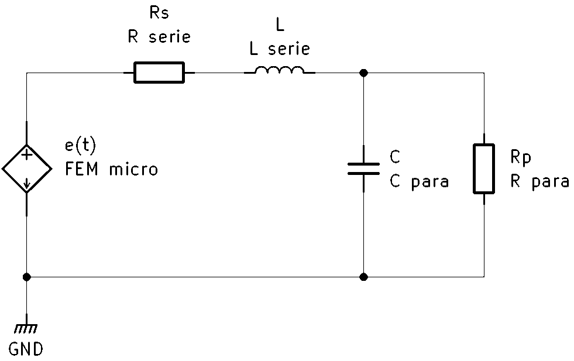
\includegraphics[width=1\textwidth]{../../../Attachment/Schema/01-Schema-eq-mic.png}
    \caption{Schéma électrique équivalent des micros}
    \label{fig:schema-mic}
\end{figure}
\end{minipage}

\newpage

\subsubsection{Calcul de la matrice Jacobienne}
\begin{lstlisting}[language=Python]
import numpy as np

def Matrice_Jacobienne(X:np.ndarray, rs:float, f:np.ndarray)->np.ndarray:
    """Basee sur l'algorythme de Levenberg_Marquardt, cette fonction retourne la matrice Jacobienne J
    Args:
        X (np.ndarray): Vecteur des caracteristique electrique interne du micro [L, C, Rp] avec L l'inductance [H], C la capacite parallèle [nF]et
            Rp la resistance parallèle [kOhm] modelisant les courants de foucauts
        rs (float):Resistance serie (DC) du micro. Peut etre mesure avec un Ohmmetre
        f (np.ndarray): Tableau des frequence f
    Returns:
        np.ndarray: Matrice Jacobienne definie tel que chaque colonne i contient les derivees partielles par rapport a la variable situe en i dans X pour toute
            pulsation w
    """
    w = 2 * np.pi * f
    L, C_n, Rp_k = X
    C, Rp = C_n * 1e-9, Rp_k * 1e3
    
    # Variables intermediaires
    den_L = rs**2 + (L * w)**2
    Y_re = (1 / Rp) + (rs / den_L)
    Y_im = (C * w) - (L * w / den_L)
    Z = 1 / np.sqrt(Y_re**2 + Y_im**2)
    Z3 = Z**3

    % Derivees partielles de Y
    dYre_dL = - (rs * 2 * L * w**2) / (den_L**2)
    dYim_dL = - (w * (rs**2 - (L * w)**2)) / (den_L**2)
    dZ_dL = - Z3 * (Y_re * dYre_dL + Y_im * dYim_dL)
    
    dYim_dCn = w * 1e-9
    dZ_dCn = - Z3 * (Y_im * dYim_dCn)

    dYre_dRpn = - 1 / (1000 * Rp_k**2)
    dZ_dRpk = - Z3 * (Y_re * dYre_dRpn)

    return np.column_stack((dZ_dL, dZ_dCn, dZ_dRpk))
\end{lstlisting}

\subsubsection{Calcul des écarts}
\begin{lstlisting}[language=Python]
import numpy as np

def residus(X:np.ndarray, rs:float, f:np.ndarray, Z_exp:np.ndarray)-> np.ndarray:
    """Calcul l'ecart (l'erreur) entre l'impedance calcule theoriquement et l'impedance reelle experimentale
    Args:
        X (np.ndarray): Vecteur des caracteristique electrique interne du micro [L, C, Rp] avec L l'inductance [H], C la capacite parallèle [nF]et
            Rp la resistance parallèle [kOhm] modelisant les courants de foucauts
        rs (float):Resistance serie (DC) du micro. Peut etre mesure avec un Ohmmetre
        f (np.ndarray): Tableau des frequence f
        Z_exp (np.ndarray): Tableau Numpy des impedances experimentale releve en Ohm
    Returns:
        np.ndarray: Tableau Numpy des distances separant chaque point theorique au point experimentaux
    """
    return Z_exp - Z_micro(X, rs, 2 * np.pi * f)
\end{lstlisting}

\subsubsection{Algorithme des moindres carrés}

\begin{figure}[H]
    \centering
    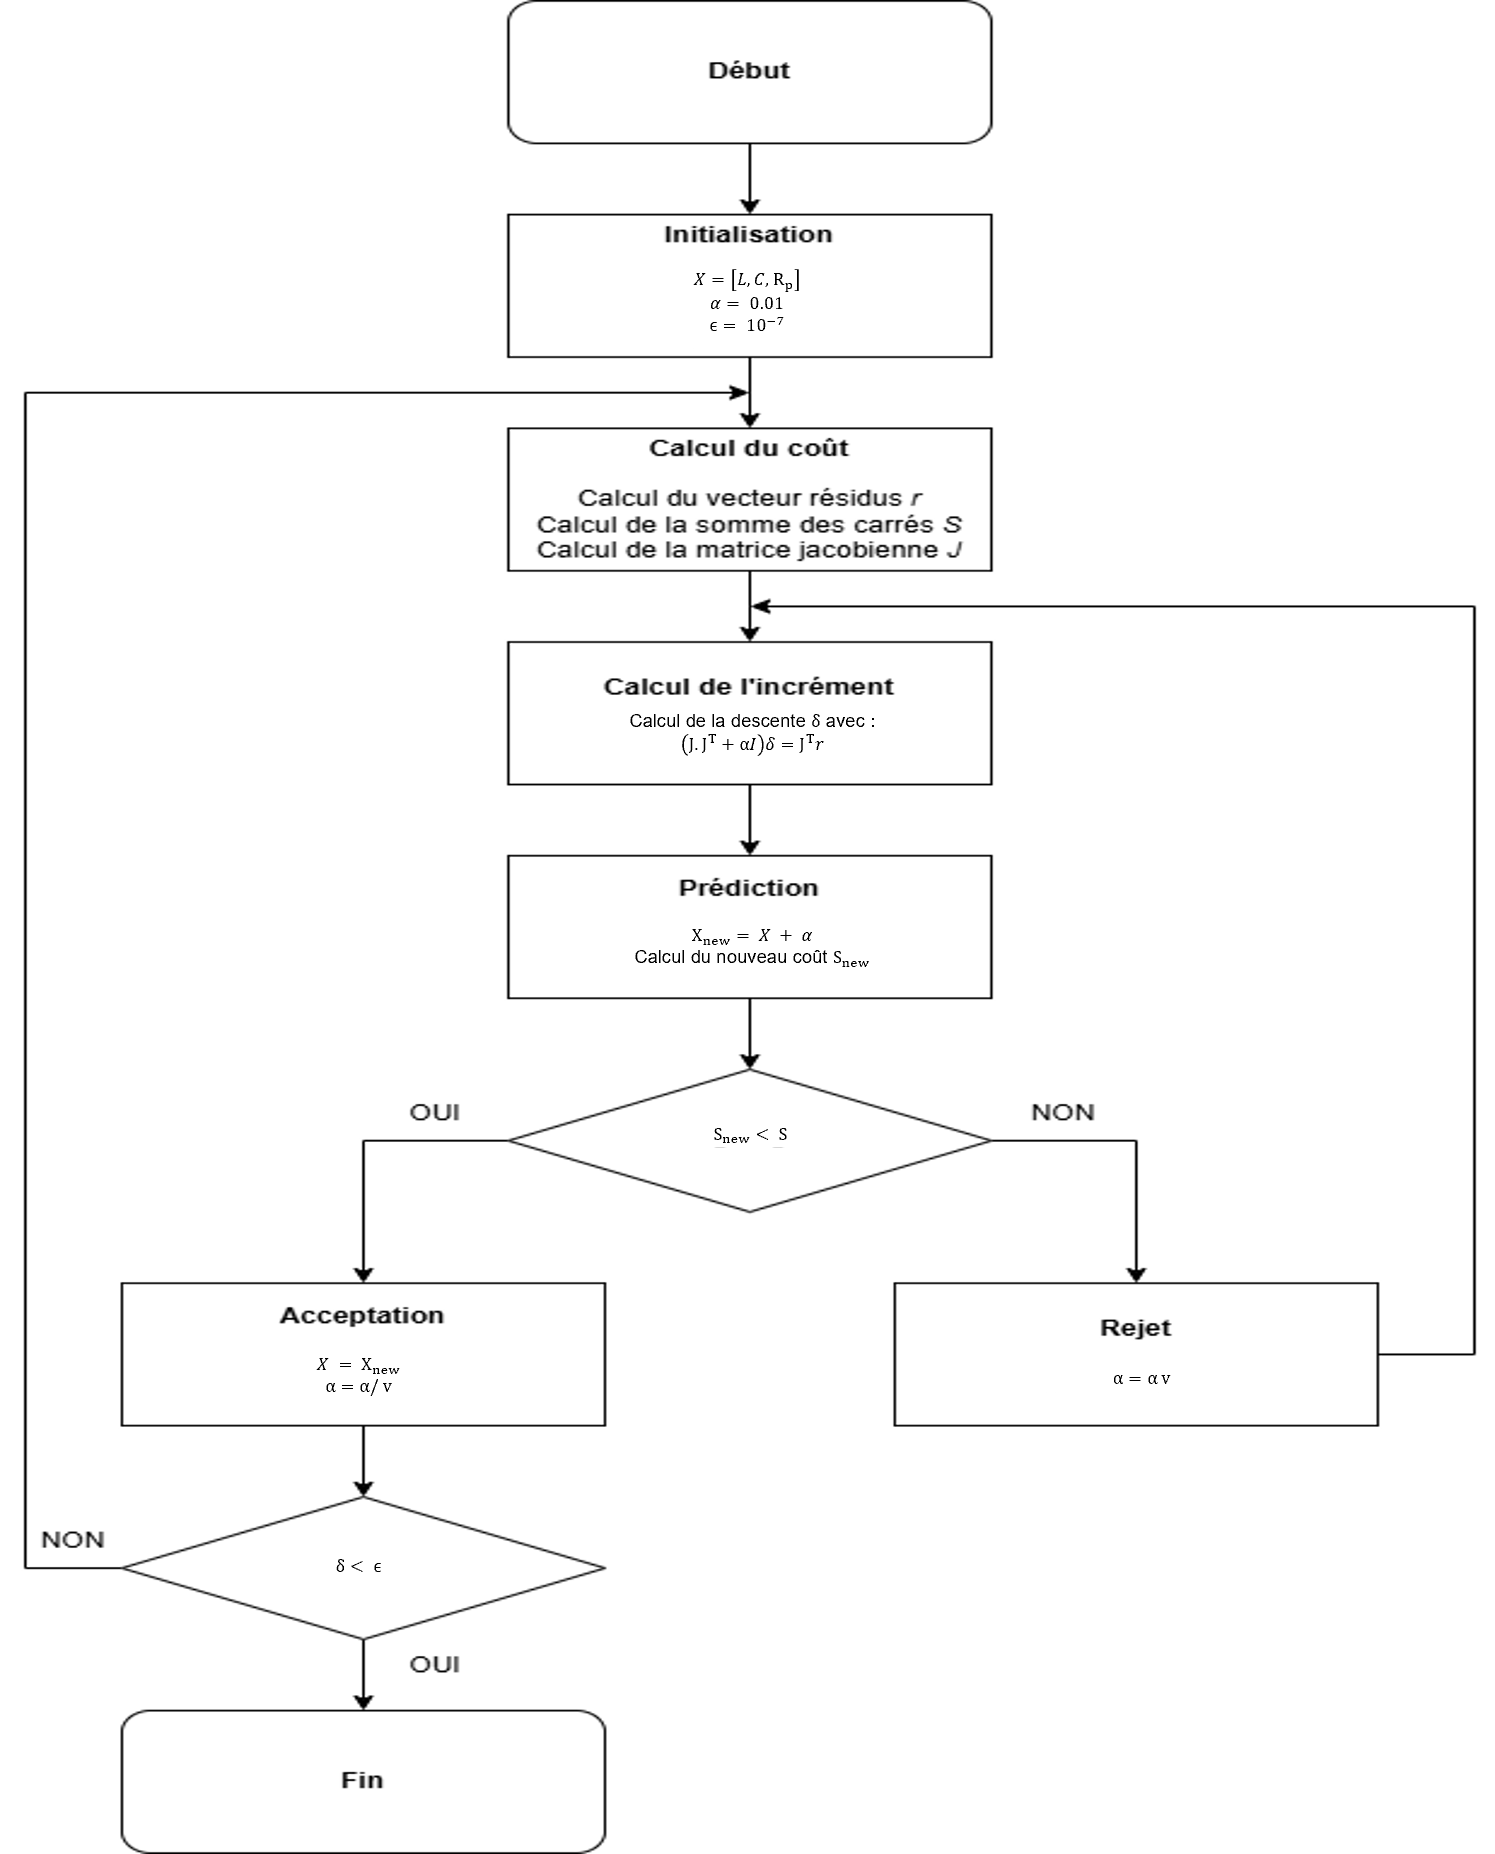
\includegraphics[width=1\textwidth]{../../../Attachment/Schema/moindre-carre.png}
    \caption{Schéma de principe de l'algorithme}
    \label{fig:schema-moindre-carre}
\end{figure}

\newpage

\begin{lstlisting}[language=Python]
import numpy as np

def Levenberg_Marquardt(X_init:np.ndarray, rs:float, f:np.ndarray, Z_exp:np.ndarray, N:int, learning_rate:float):
    """Algorythme de Levenberg-Marquardt pour l'optimisation non-lineaire des parametres electriques du micro

    Args:
        X_init (np.ndarray): Vecteur initial des caracteristique electrique interne du micro [L, C, Rp] avec L l'inductance [H], C la capacite parallèle [nF]et
            Rp la resistance parallèle [kOhm] modelisant les courants de foucauts
        rs (float): Resistance serie (DC) du micro. Peut etre mesure avec un Ohmmetre
        f (np.ndarray): Tableau des frequence f
        Z_exp (np.ndarray): Tableau Numpy des impedances experimentale releve en Ohm
        N (int): Nombre d'iterations de l'algorithme

    Returns:
        np.ndarray: Vecteur optimisé des caracteristique electrique interne du micro [L, C, Rp] avec L l'inductance [H], C la capacite parallèle [nF]et
            Rp la resistance parallèle [kOhm] modelisant les courants de foucauts
    """
    X = np.array(X_init, dtype=float)
    alpha = learning_rate
    v = 3
    r = None
    eps = None
    
    for _ in range(N):
        r = residus(X, rs, f, Z_exp)
        eps = np.sum(r**2)
        J = Matrice_Jacobienne(X, rs, f)

        H = J.T @ J
        g = J.T @ r
        
        # Amortissement de Marquardt
        H_lm = H + alpha * np.diag(np.diag(H) + 1e-8)
        
        try:
            delta = np.linalg.solve(H_lm, g)
        except np.linalg.LinAlgError:
            break

        X_new = X + delta
        # Contrainte physique : paramètres toujours positifs
        X_new = np.maximum(X_new, [1e-2, 1e-2, 1e-2]) 
        eps_new = np.sum(residus(X_new, rs, f, Z_exp)**2)
        if eps_new < eps:
            alpha /= v
            X = X_new
            if np.linalg.norm(delta) / np.linalg.norm(X) < 1e-12:
                break
        else:
            alpha *= v
            
    return X, eps_new
\end{lstlisting}

\subsubsection{Calcul du diagramme de Bode}
\begin{minipage}{\textwidth}
\begin{lstlisting}[language=Python]
import numpy as np

def calcul_bode(X:np.ndarray, rs:float, f:np.ndarray, Ramp:float=1e6)-> tuple[np.ndarray, np.ndarray]:
    """Calcul la fonction de transfert en gain et phase d'un micro de guitare en fonction de ses parametres internes
    Args:
        X (np.ndarray): Vecteur optimisé des caracteristique electrique interne du micro [L, C, Rp] avec L l'inductance [H], C la capacite parallèle [nF]et
            Rp la resistance parallèle [kOhm] modelisant les courants de foucauts
        rs (float): Resistance serie (DC) du micro. Peut etre mesure avec un Ohmmetre
        f (np.ndarray): Tableau des frequence f
        Ramp (float, optional): Resistance d'entree de l'amplificateur. Defaults to 1e6.
    Returns:
        tuple[np.ndarray, np.ndarray]: Deux tableaux Numpy contenant respectivement le gain (en dB) et la phase (en degres) de la fonction de transfert du micro
    """
    w = 2 * np.pi * f
    L, C, Rp = X[0], X[1] * 1e-9, X[2] * 1e3
    
    # Impedance serie
    Z_ser = rs + 1j * L * w
    
    # Impedance parallèle
    Y_para = (1 / Rp) + (1 / Ramp) + (1j * C * w)
    Z_para = 1 / Y_para
    
    # Fonction de transfert
    H = Z_para / (Z_ser + Z_para)
    
    gain = 20 * np.log10(np.abs(H))
    phase = np.angle(H, deg=True)
    return gain, phase
\end{lstlisting}
\end{minipage}

\begin{figure}[H]
    \centering
    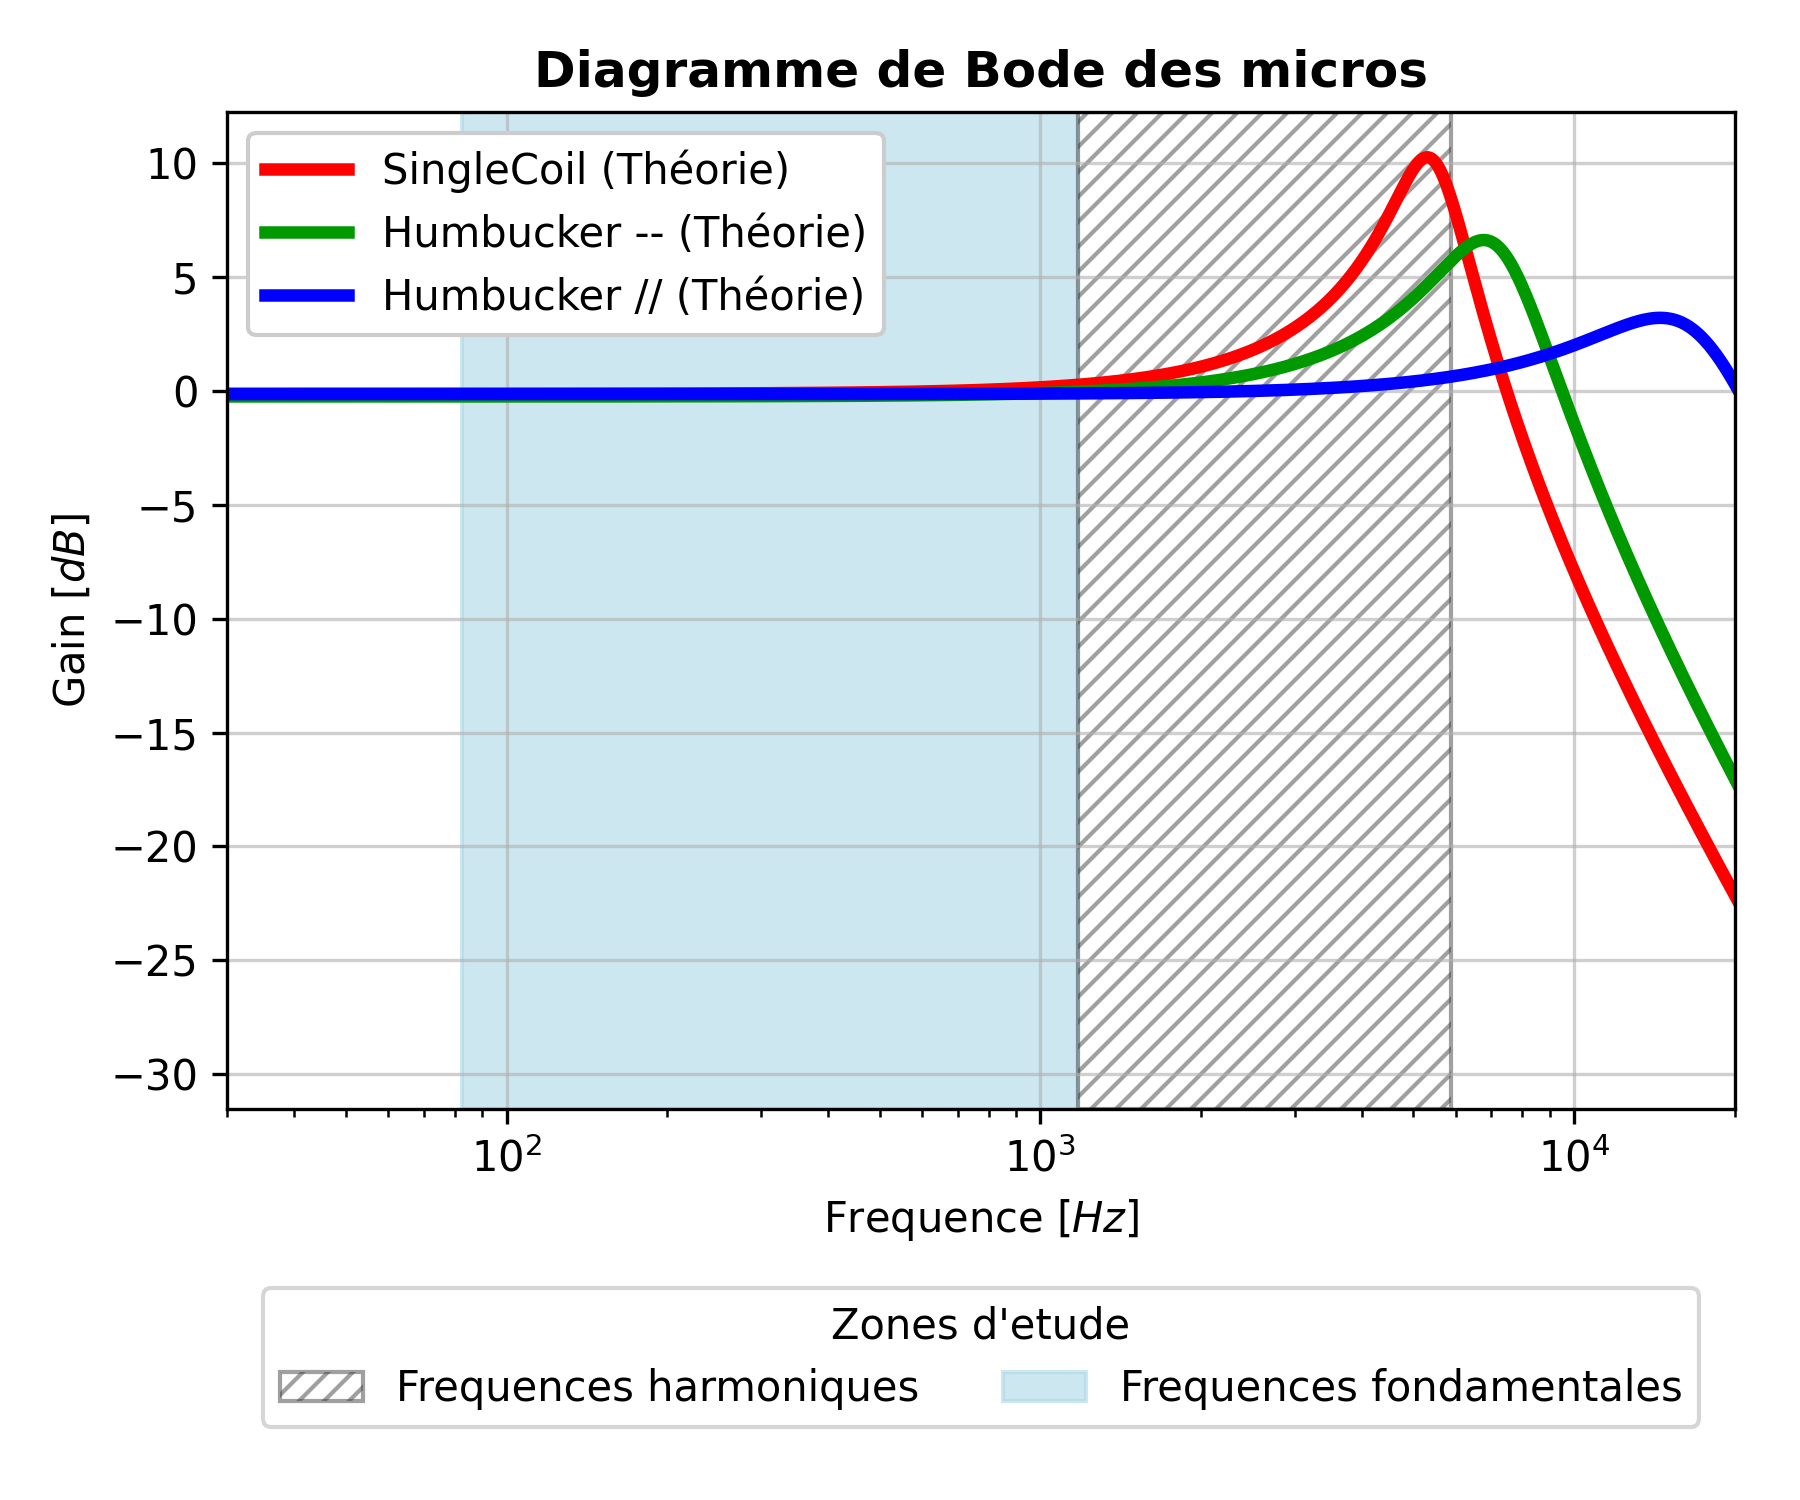
\includegraphics[width=0.8\textwidth]{../../Exports/01-Reponse_electrique_frequetielle/01-Gain.png}
    \caption{Diagramme de Bode des micros}
    \label{fig:bode-micro}
\end{figure}

\subsection{Mise en évidence du filtrage spatial}
\begin{minipage}{\textwidth}
\begin{lstlisting}[language=Python]
import numpy as np
from scipy.signal import find_peaks

def extraire_pics_separes(frequences, amplitudes, prominence=0.05, distance=10):
    """Extrait les pics significatifs d'un spectre de Fourier en utilisant la proeminence."""
    indices, _ = find_peaks(amplitudes, prominence=prominence, distance=distance)
    liste_frequences = frequences[indices].tolist()
    liste_amplitudes = amplitudes[indices].tolist()
    return np.array(liste_frequences), np.round(liste_amplitudes, 3)

kw_peigne = {'color': "#000000", 'label': 'Peigne spatial', 'linewidth': 3}
kw_att = {'color': "#888888", 'label': 'Gain relatif', 'linewidth': 1}

L_freqs, L_pic_s_exp = mod.extraire_pics_separes(freqs_s_exp, fft_s_exp, prominence=0.04, distance=5)
L_freqs, L_pic_hs_exp = mod.extraire_pics_separes(freqs_hs_exp, fft_hs_exp, prominence=0.03, distance=5)

freqs = np.linspace(30, 20000, 1000)
signal_hs, peigne_hs, signal_sc = mod.attenuation_theorique_db(freqs, x_hs1, x_hs2)
signal_hp, peigne_hp, signal_sc = mod.attenuation_theorique_db(freqs, x_hp1, x_hp2)

Attenuation_th = 20*np.log10(np.abs(signal_hs / (signal_sc + 1e-6)) + 1e-6)
Attenuation_exp = 20*np.log10(np.abs(L_pic_hs_exp / (L_pic_s_exp + 1e-6)) + 1e-6)
mod.save_plot(PATH_exp + "Filtrage_spatial.png",
        (freqs, Attenuation_th, kw_att),
        (L_freqs, Attenuation_exp, kw_Hs_exp),
        (freqs, 20*np.log10(np.abs(peigne_hs)+1e-6), kw_peigne),
        title=f"Filtrage spatial du micro Humbucker série", 
        xlabel="Frequence [$Hz$]", ylabel="Gain [dB]", xlim=(30, 20000), vspan=True,
        log=True)
\end{lstlisting}
\end{minipage} % La minipage se ferme BIEN ICI, avant la figure.

\begin{figure}[H]
    \centering
    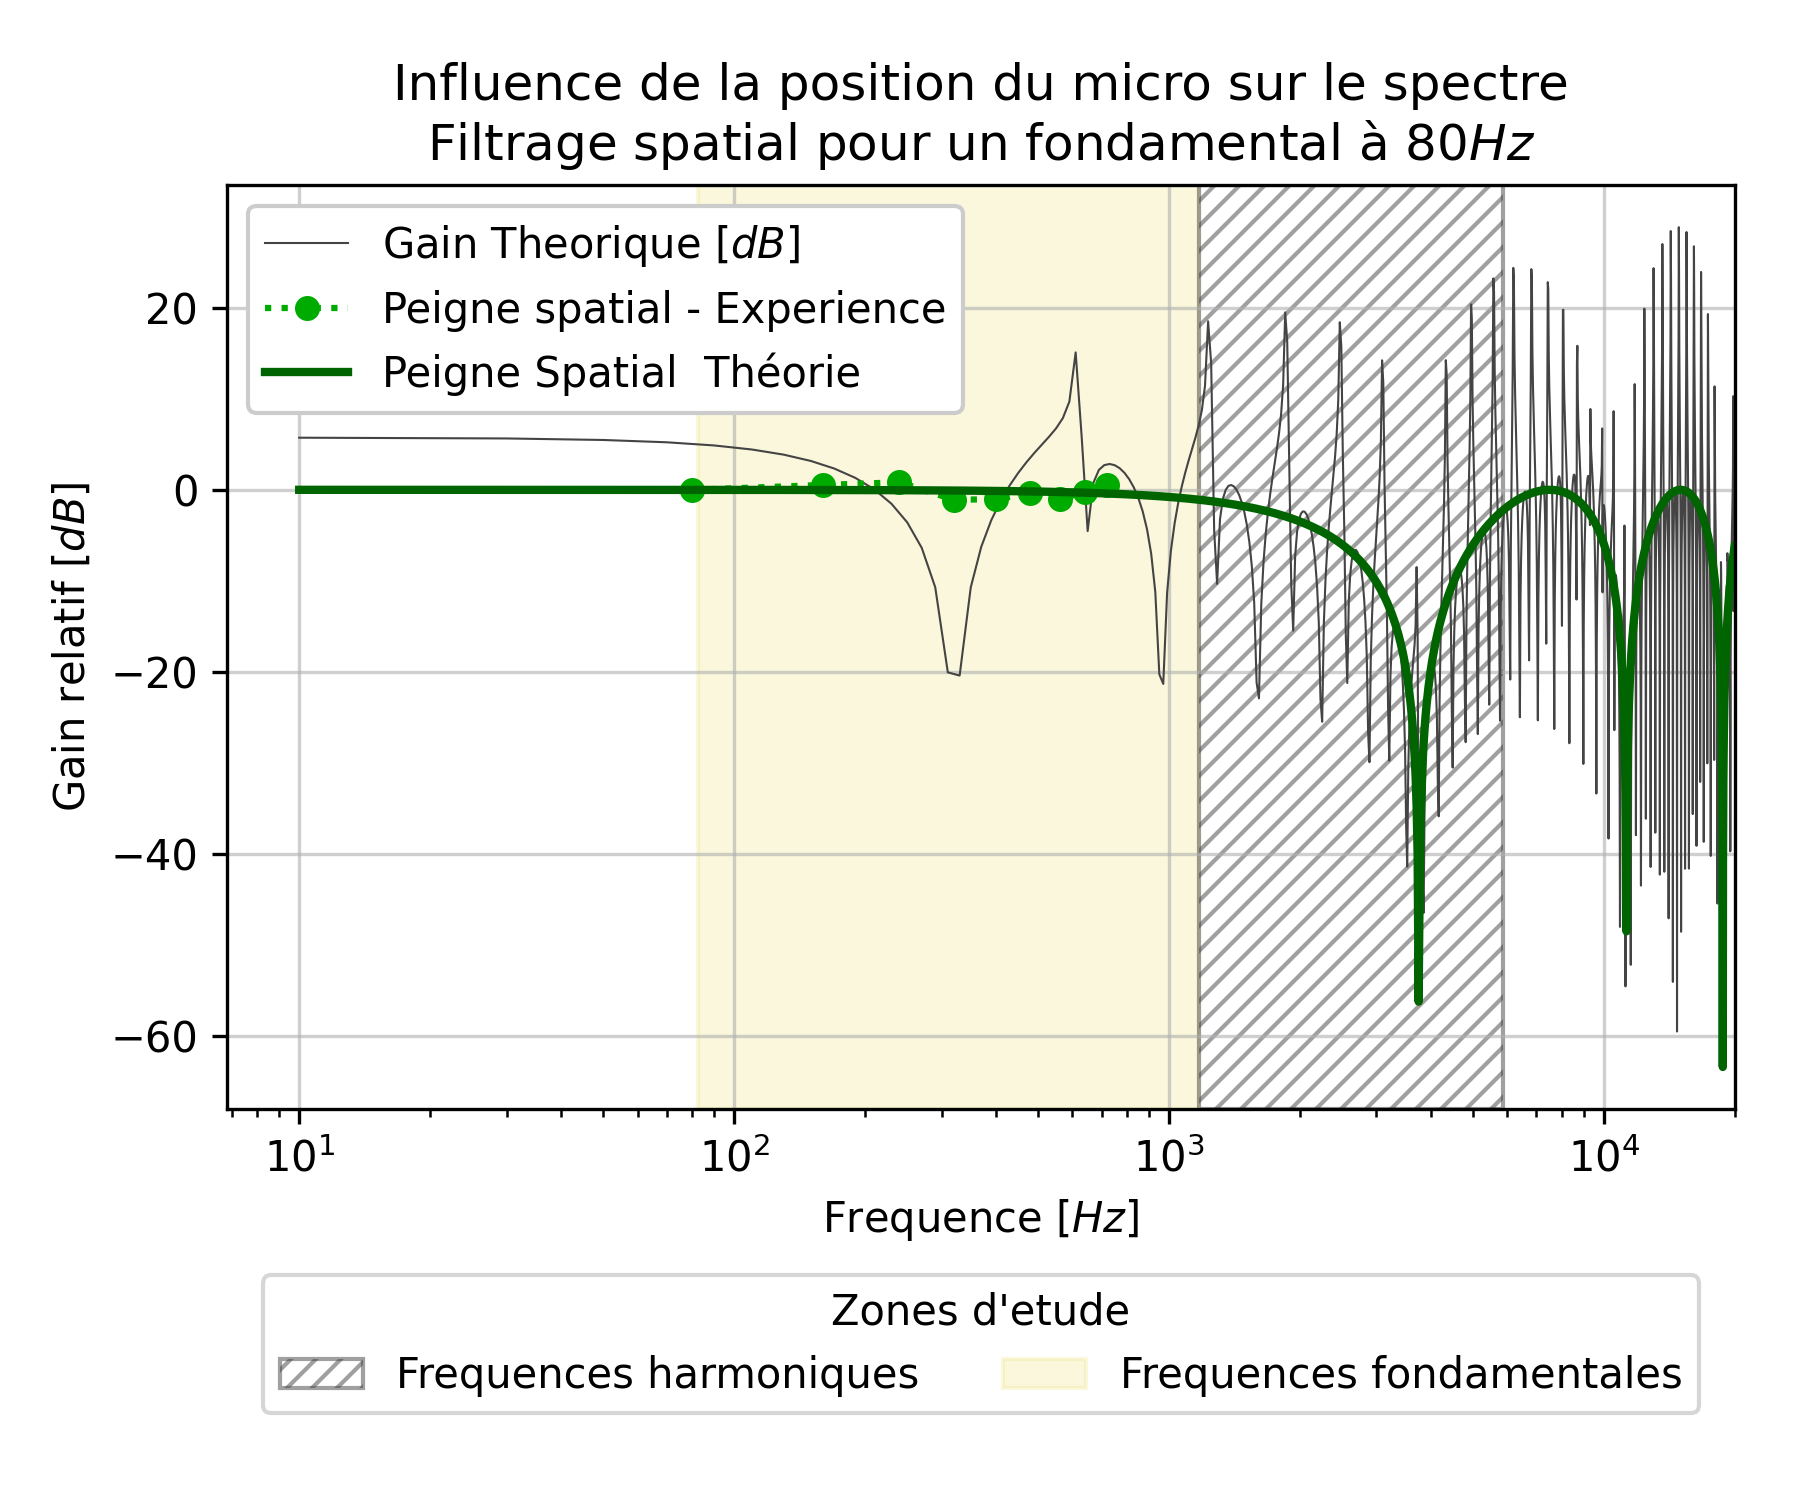
\includegraphics[width=0.8\textwidth]{../../Exports/02-Reponse_mecanique/Filtrage_spatial.png}
    \caption{Filtrage spatial du Humbucker série}
    \label{fig:filtre-spatial}
\end{figure}

\newpage

% ==============================================================================
\section{Traitement des données expérimentales}
% ==============================================================================

\subsection{Filtrage des données (Passe-bas numérique)}
\begin{lstlisting}[language=Python]
import numpy as np

def lire_fichier(PATH):
    List_temps = []
    List_sig = []
    file_s2 = open(PATH)
    L_lignes = file_s2.readlines()

    for ligne in L_lignes[2:]:
        ligne = ligne.strip().split(',')
        ligne = [x.replace('\n', '') for x in ligne]
        ligne = [x.replace('E', 'e') for x in ligne]
        List_temps.append(float(ligne[0]))
        List_sig.append(float(ligne[1]))
    
    return List_temps, List_sig

def write_file(PATH, List_temps, List_sig):
    with open(PATH, 'w') as file:
        file.write('Time;Signal\n')
        for t, s in zip(List_temps, List_sig):
            file.write(f"{t}\t{s}\n")

def filtre_passe_bas_1er_ordre(List_temps, List_sig, tau=0.001):
    """Filtre passe-bas du 1er ordre (IIR)."""
    sig_array = np.array(List_sig)

    if tau < 0:
        tau = 0.001

    if len(List_temps) > 1:
        dt = (List_temps[-1] - List_temps[0]) / (len(List_temps) - 1)
    else:
        dt = 1.0

    alpha = dt / (tau + dt)

    filtered_sig = np.zeros_like(sig_array)
    filtered_sig[0] = sig_array[0]
    for i in range(1, len(sig_array)):
        filtered_sig[i] = alpha * sig_array[i] + (1 - alpha) * filtered_sig[i - 1]

    return filtered_sig
\end{lstlisting}

\subsection{Amplitude d'un signal périodique}
\begin{lstlisting}[language=Python]
def get_amplitude(PATH):
    List_temps = []
    List_sig = []
    file = open(PATH)
    
    L_lignes = file.readlines()
    for ligne in L_lignes[1:70000]:
        ligne = ligne.strip().split('\t')
        ligne = [x.replace('\n', '') for x in ligne]
        ligne = [x.replace(',', '.') for x in ligne]
        List_temps.append(float(ligne[0]))
        List_sig.append(float(ligne[1]))
    
    amplitude = max(List_sig) - min(List_sig)
    return amplitude
\end{lstlisting}

\newpage
% ==============================================================================
\section{Données et valeurs numériques}
% ==============================================================================

\subsection{Caractéristiques électriques et mécaniques}
\begin{center}
\small
\begin{tabularx}{\textwidth}{llcX}
\toprule
\textbf{Notation} & \textbf{Valeur} & \textbf{Unité} & \textbf{Description} \\
\midrule
$\mu_{0}$ & $4\pi \cdot 10^{-7}$ & H$\cdot$m$^{-1}$ & Perméabilité magnétique du vide \\
$\mu_{r}$ & 2 & -- & Perméabilité relative de l'Alnico 5 \\
$e(t)$ & -- & V & Force électromotrice (f.e.m.) induite dans le micro \\
$u(t)$ & -- & V & Tension en sortie du micro chargé \\
$u_{\text{GBF}}(t)$ & -- & V & Tension délivrée par le générateur de fonction \\
$H(p)$ & -- & -- & Fonction de transfert du circuit de filtrage \\
\midrule
$R_{s_S}$ & $5,26 \cdot 10^3$ & $\Omega$ & Résistance interne du micro SingleCoil \\
$L_{S}$ & 2,43 & H & Inductance du micro SingleCoil \\
$C_{S}$ & $360 \cdot 10^{-12}$ & F & Capacité interne du micro SingleCoil \\
$R_{p_S}$ & $500 \cdot 10^3$ & $\Omega$ & Résistance des pertes par courant de Foucault \\
$Z_{S}(\omega)$ & -- & $\Omega$ & Impédance complexe du micro SingleCoil \\
\midrule
$R_{s_{\text{Hp}}}$ & $4,52 \cdot 10^3$ & $\Omega$ & Résistance interne du micro Humbucker parallèle \\
$L_{\text{Hp}}$ & 1,77 & H & Inductance du micro Humbucker parallèle \\
$C_{\text{Hp}}$ & $50 \cdot 10^{-12}$ & F & Capacité interne du micro Humbucker parallèle \\
$R_{p_{\text{Hp}}}$ & $351 \cdot 10^3$ & $\Omega$ & Résistance des pertes par courant de Foucault \\
$Z_{\text{Hp}}(\omega)$ & -- & $\Omega$ & Impédance complexe du micro Humbucker parallèle \\
\midrule
$R_{s_{\text{Hs}}}$ & $15,10 \cdot 10^3$ & $\Omega$ & Résistance interne du micro Humbucker série \\
$L_{\text{Hs}}$ & 4,71 & H & Inductance du micro Humbucker série \\
$C_{\text{Hs}}$ & $110 \cdot 10^{-12}$ & F & Capacité interne du micro Humbucker série \\
$R_{p_{\text{Hs}}}$ & $1,07 \cdot 10^6$ & $\Omega$ & Résistance des pertes par courant de Foucault \\
$Z_{\text{Hs}}(\omega)$ & -- & $\Omega$ & Impédance complexe du micro Humbucker série \\
\midrule
$z(x,t)$ & -- & m & Déplacement vertical de la corde \\
$z_{0}$ & 0,004 & m & Distance corde micro au repos \\
$L$ & 0,85 & m & Longueur de la corde vibrante \\
$x_{0}$ & 0,300 & m & Position de l'origine de la perturbation \\
$A_{0}$ & 0,001 & m & Amplitude initiale de la perturbation \\
$B_{n}$ & -- & m & Amplitude de l'harmonique de rang n \\
$F$ & 80 & Hz & Fréquence fondamentale de vibration de la corde \\
$m$ & -- & A$\cdot$m$^{2}$ & Moment dipolaire de la corde \\
\bottomrule
\end{tabularx}
\end{center}

\newpage

\subsection{Caractéristiques magnétiques}
\begin{center}
\small
\begin{tabularx}{\textwidth}{llcX}
\toprule
\textbf{Notation} & \textbf{Valeur} & \textbf{Unité} & \textbf{Description} \\
\midrule
$\Phi(z,t)$ & -- & Wb & Flux magnétique traversant la bobine \\
$\chi$ & 100 (ODG) & -- & Susceptibilité magnétique de la corde \\
$V$ & $1 \cdot 10^{-8}$ (ODG) & m$^{3}$ & Volume de la portion de la corde active \\
$B_{m}(z)$ & -- & T & Champ magnétique statique des micros \\
$B_{c}(z)$ & -- & T & Champ magnétique induit par le moment dipolaire \\
\midrule
$x_{S}$ & 0,105 & m & Position du micro SingleCoil \\
$x_{\text{Hp1}}, x_{\text{Hp2}}$ & 0,147 - 0,165 & m & Position des bobinages du Humbucker parallèle \\
$x_{\text{Hs1}}, x_{\text{Hs2}}$ & 0,202 - 0,220 & m & Position des bobinages du Humbucker série \\
$\Delta$ & 0,018 & m & Entraxe entre les deux bobines du Humbucker \\
\midrule
$F_{B}$ & 50 & Hz & Fréquence du champ magnétique parasite \\
$B_{0}$ & -- & T & Amplitude du champ magnétique parasite \\
$\alpha$ & 2 (ODG) & m$^{-1}$ & Gradient du champ magnétique parasite \\
\midrule
$k_{s}$ & 1,46 & $\mu$T$^{-1}$ & Sensibilité théorique du SingleCoil \\
$k_{\text{Hp}}$ & 0,02 & $\mu$T$^{-1}$ & Sensibilité théorique du Humbucker parallèle \\
$k_{\text{Hs}}$ & -- & $\mu$T$^{-1}$ & Sensibilité théorique du Humbucker série \\
$k_{\text{Sexp}}$ & 1,48 & $\mu$T$^{-1}$ & Sensibilité expérimentale du SingleCoil \\
$k_{\text{Hpexp}}$ & 0,62 & $\mu$T$^{-1}$ & Sensibilité expérimentale du Humbucker parallèle \\
$k_{\text{Hsexp}}$ & -- & $\mu$T$^{-1}$ & Sensibilité expérimentale du Humbucker série \\
\midrule
$\text{CMRR}$ & 37 & dB & CMRR théorique du Humbucker \\
$\text{CMRR}_{\text{Hpexp}}$ & 7,6 & dB & CMRR expérimentale du Humbucker parallèle \\
$\text{CMRR}_{\text{Hsexp}}$ & -- & dB & CMRR expérimentale du Humbucker série \\
\bottomrule
\end{tabularx}
\end{center}

\end{document}